
%% bare_conf.tex
%% V1.4b
%% 2015/08/26
%% by Michael Shell
%% See:
%% http://www.michaelshell.org/
%% for current contact information.
%%
%% This is a skeleton file demonstrating the use of IEEEtran.cls
%% (requires IEEEtran.cls version 1.8b or later) with an IEEE
%% conference paper.
%%
%% Support sites:
%% http://www.michaelshell.org/tex/ieeetran/
%% http://www.ctan.org/pkg/ieeetran
%% and
%% http://www.ieee.org/

%%*************************************************************************


% *** Authors should verify (and, if needed, correct) their LaTeX system  ***
% *** with the testflow diagnostic prior to trusting their LaTeX platform ***
% *** with production work. The IEEE's font choices and paper sizes can   ***
% *** trigger bugs that do not appear when using other class files.       ***                          ***
% The testflow support page is at:
% http://www.michaelshell.org/tex/testflow/



\documentclass[conference]{IEEEtran}
% Some Computer Society conferences also require the compsoc mode option,
% but others use the standard conference format.
%
% If IEEEtran.cls has not been installed into the LaTeX system files,
% manually specify the path to it like:
% \documentclass[conference]{../sty/IEEEtran}





% Some very useful LaTeX packages include:
% (uncomment the ones you want to load)


% *** MISC UTILITY PACKAGES ***
%
%\usepackage{ifpdf}
% Heiko Oberdiek's ifpdf.sty is very useful if you need conditional
% compilation based on whether the output is pdf or dvi.
% usage:
% \ifpdf
%   % pdf code
% \else
%   % dvi code
% \fi
% The latest version of ifpdf.sty can be obtained from:
% http://www.ctan.org/pkg/ifpdf
% Also, note that IEEEtran.cls V1.7 and later provides a builtin
% \ifCLASSINFOpdf conditional that works the same way.
% When switching from latex to pdflatex and vice-versa, the compiler may
% have to be run twice to clear warning/error messages.






% *** CITATION PACKAGES ***
%
\usepackage{cite}
% cite.sty was written by Donald Arseneau
% V1.6 and later of IEEEtran pre-defines the format of the cite.sty package
% \cite{} output to follow that of the IEEE. Loading the cite package will
% result in citation numbers being automatically sorted and properly
% "compressed/ranged". e.g., [1], [9], [2], [7], [5], [6] without using
% cite.sty will become [1], [2], [5]--[7], [9] using cite.sty. cite.sty's
% \cite will automatically add leading space, if needed. Use cite.sty's
% noadjust option (cite.sty V3.8 and later) if you want to turn this off
% such as if a citation ever needs to be enclosed in parenthesis.
% cite.sty is already installed on most LaTeX systems. Be sure and use
% version 5.0 (2009-03-20) and later if using hyperref.sty.
% The latest version can be obtained at:
% http://www.ctan.org/pkg/cite
% The documentation is contained in the cite.sty file itself.






% *** GRAPHICS RELATED PACKAGES ***
%
\ifCLASSINFOpdf
  % \usepackage[pdftex]{graphicx}
  % declare the path(s) where your graphic files are
  % \graphicspath{{../pdf/}{../jpeg/}}
  % and their extensions so you won't have to specify these with
  % every instance of \includegraphics
  % \DeclareGraphicsExtensions{.pdf,.jpeg,.png}
\else
  % or other class option (dvipsone, dvipdf, if not using dvips). graphicx
  % will default to the driver specified in the system graphics.cfg if no
  % driver is specified.
  % \usepackage[dvips]{graphicx}
  % declare the path(s) where your graphic files are
  % \graphicspath{{../eps/}}
  % and their extensions so you won't have to specify these with
  % every instance of \includegraphics
  % \DeclareGraphicsExtensions{.eps}
\fi
% graphicx was written by David Carlisle and Sebastian Rahtz. It is
% required if you want graphics, photos, etc. graphicx.sty is already
% installed on most LaTeX systems. The latest version and documentation
% can be obtained at: 
% http://www.ctan.org/pkg/graphicx
% Another good source of documentation is "Using Imported Graphics in
% LaTeX2e" by Keith Reckdahl which can be found at:
% http://www.ctan.org/pkg/epslatex
%
% latex, and pdflatex in dvi mode, support graphics in encapsulated
% postscript (.eps) format. pdflatex in pdf mode supports graphics
% in .pdf, .jpeg, .png and .mps (metapost) formats. Users should ensure
% that all non-photo figures use a vector format (.eps, .pdf, .mps) and
% not a bitmapped formats (.jpeg, .png). The IEEE frowns on bitmapped formats
% which can result in "jaggedy"/blurry rendering of lines and letters as
% well as large increases in file sizes.
%
% You can find documentation about the pdfTeX application at:
% http://www.tug.org/applications/pdftex
\usepackage{graphicx}
\usepackage{caption}
\usepackage{subcaption}
\graphicspath{{./images/}}
\usepackage{float}
\usepackage{scrextend}
\usepackage{url}

\usepackage{booktabs}
%\usepackage{hyperref}



% *** MATH PACKAGES ***
%
%\usepackage{amsmath}
% A popular package from the American Mathematical Society that provides
% many useful and powerful commands for dealing with mathematics.
%
% Note that the amsmath package sets \interdisplaylinepenalty to 10000
% thus preventing page breaks from occurring within multiline equations. Use:
%\interdisplaylinepenalty=2500
% after loading amsmath to restore such page breaks as IEEEtran.cls normally
% does. amsmath.sty is already installed on most LaTeX systems. The latest
% version and documentation can be obtained at:
% http://www.ctan.org/pkg/amsmath





% *** SPECIALIZED LIST PACKAGES ***
%
%\usepackage{algorithmic}
% algorithmic.sty was written by Peter Williams and Rogerio Brito.
% This package provides an algorithmic environment fo describing algorithms.
% You can use the algorithmic environment in-text or within a figure
% environment to provide for a floating algorithm. Do NOT use the algorithm
% floating environment provided by algorithm.sty (by the same authors) or
% algorithm2e.sty (by Christophe Fiorio) as the IEEE does not use dedicated
% algorithm float types and packages that provide these will not provide
% correct IEEE style captions. The latest version and documentation of
% algorithmic.sty can be obtained at:
% http://www.ctan.org/pkg/algorithms
% Also of interest may be the (relatively newer and more customizable)
% algorithmicx.sty package by Szasz Janos:
% http://www.ctan.org/pkg/algorithmicx




% *** ALIGNMENT PACKAGES ***
%
%\usepackage{array}
% Frank Mittelbach's and David Carlisle's array.sty patches and improves
% the standard LaTeX2e array and tabular environments to provide better
% appearance and additional user controls. As the default LaTeX2e table
% generation code is lacking to the point of almost being broken with
% respect to the quality of the end results, all users are strongly
% advised to use an enhanced (at the very least that provided by array.sty)
% set of table tools. array.sty is already installed on most systems. The
% latest version and documentation can be obtained at:
% http://www.ctan.org/pkg/array


% IEEEtran contains the IEEEeqnarray family of commands that can be used to
% generate multiline equations as well as matrices, tables, etc., of high
% quality.




% *** SUBFIGURE PACKAGES ***
%\ifCLASSOPTIONcompsoc
%  \usepackage[caption=false,font=normalsize,labelfont=sf,textfont=sf]{subfig}
%\else
%  \usepackage[caption=false,font=footnotesize]{subfig}
%\fi
% subfig.sty, written by Steven Douglas Cochran, is the modern replacement
% for subfigure.sty, the latter of which is no longer maintained and is
% incompatible with some LaTeX packages including fixltx2e. However,
% subfig.sty requires and automatically loads Axel Sommerfeldt's caption.sty
% which will override IEEEtran.cls' handling of captions and this will result
% in non-IEEE style figure/table captions. To prevent this problem, be sure
% and invoke subfig.sty's "caption=false" package option (available since
% subfig.sty version 1.3, 2005/06/28) as this is will preserve IEEEtran.cls
% handling of captions.
% Note that the Computer Society format requires a larger sans serif font
% than the serif footnote size font used in traditional IEEE formatting
% and thus the need to invoke different subfig.sty package options depending
% on whether compsoc mode has been enabled.
%
% The latest version and documentation of subfig.sty can be obtained at:
% http://www.ctan.org/pkg/subfig




% *** FLOAT PACKAGES ***
%
%\usepackage{fixltx2e}
% fixltx2e, the successor to the earlier fix2col.sty, was written by
% Frank Mittelbach and David Carlisle. This package corrects a few problems
% in the LaTeX2e kernel, the most notable of which is that in current
% LaTeX2e releases, the ordering of single and double column floats is not
% guaranteed to be preserved. Thus, an unpatched LaTeX2e can allow a
% single column figure to be placed prior to an earlier double column
% figure.
% Be aware that LaTeX2e kernels dated 2015 and later have fixltx2e.sty's
% corrections already built into the system in which case a warning will
% be issued if an attempt is made to load fixltx2e.sty as it is no longer
% needed.
% The latest version and documentation can be found at:
% http://www.ctan.org/pkg/fixltx2e


%\usepackage{stfloats}
% stfloats.sty was written by Sigitas Tolusis. This package gives LaTeX2e
% the ability to do double column floats at the bottom of the page as well
% as the top. (e.g., "\begin{figure*}[!b]" is not normally possible in
% LaTeX2e). It also provides a command:
%\fnbelowfloat
% to enable the placement of footnotes below bottom floats (the standard
% LaTeX2e kernel puts them above bottom floats). This is an invasive package
% which rewrites many portions of the LaTeX2e float routines. It may not work
% with other packages that modify the LaTeX2e float routines. The latest
% version and documentation can be obtained at:
% http://www.ctan.org/pkg/stfloats
% Do not use the stfloats baselinefloat ability as the IEEE does not allow
% \baselineskip to stretch. Authors submitting work to the IEEE should note
% that the IEEE rarely uses double column equations and that authors should try
% to avoid such use. Do not be tempted to use the cuted.sty or midfloat.sty
% packages (also by Sigitas Tolusis) as the IEEE does not format its papers in
% such ways.
% Do not attempt to use stfloats with fixltx2e as they are incompatible.
% Instead, use Morten Hogholm'a dblfloatfix which combines the features
% of both fixltx2e and stfloats:
%
% \usepackage{dblfloatfix}
% The latest version can be found at:
% http://www.ctan.org/pkg/dblfloatfix




% *** PDF, URL AND HYPERLINK PACKAGES ***
%
%\usepackage{url}
% url.sty was written by Donald Arseneau. It provides better support for
% handling and breaking URLs. url.sty is already installed on most LaTeX
% systems. The latest version and documentation can be obtained at:
% http://www.ctan.org/pkg/url
% Basically, \url{my_url_here}.




% *** Do not adjust lengths that control margins, column widths, etc. ***
% *** Do not use packages that alter fonts (such as pslatex).         ***
% There should be no need to do such things with IEEEtran.cls V1.6 and later.
% (Unless specifically asked to do so by the journal or conference you plan
% to submit to, of course. )


% correct bad hyphenation here
\hyphenation{op-tical net-works semi-conduc-tor}


\begin{document}
%
% paper title
% Titles are generally capitalized except for words such as a, an, and, as,
% at, but, by, for, in, nor, of, on, or, the, to and up, which are usually
% not capitalized unless they are the first or last word of the title.
% Linebreaks \\ can be used within to get better formatting as desired.
% Do not put math or special symbols in the title.
\title{Subword Spotting for Use in a\\Computer Assisted Transcription System}


% author names and affiliations
% use a multiple column layout for up to three different
% affiliations
\author{\IEEEauthorblockN{Brian Davis, Robert Clawson and William Barrett}
\IEEEauthorblockA{Brigham Young University, Provo, Utah\\
Email: briandavis@byu.net}
%\and
%\IEEEauthorblockN{Homer Simpson}
%\IEEEauthorblockA{Twentieth Century Fox\\
%Springfield, USA\\
%Email: homer@thesimpsons.com}
}

% conference papers do not typically use \thanks and this command
% is locked out in conference mode. If really needed, such as for
% the acknowledgment of grants, issue a \IEEEoverridecommandlockouts
% after \documentclass

% for over three affiliations, or if they all won't fit within the width
% of the page, use this alternative format:
% 
%\author{\IEEEauthorblockN{Michael Shell\IEEEauthorrefmark{1},
%Homer Simpson\IEEEauthorrefmark{2},
%James Kirk\IEEEauthorrefmark{3}, 
%Montgomery Scott\IEEEauthorrefmark{3} and
%Eldon Tyrell\IEEEauthorrefmark{4}}
%\IEEEauthorblockA{\IEEEauthorrefmark{1}School of Electrical and Computer Engineering\\
%Georgia Institute of Technology,
%Atlanta, Georgia 30332--0250\\ Email: see http://www.michaelshell.org/contact.html}
%\IEEEauthorblockA{\IEEEauthorrefmark{2}Twentieth Century Fox, Springfield, USA\\
%Email: homer@thesimpsons.com}
%\IEEEauthorblockA{\IEEEauthorrefmark{3}Starfleet Academy, San Francisco, California 96678-2391\\
%Telephone: (800) 555--1212, Fax: (888) 555--1212}
%\IEEEauthorblockA{\IEEEauthorrefmark{4}Tyrell Inc., 123 Replicant Street, Los Angeles, California 90210--4321}}




% use for special paper notices
%\IEEEspecialpapernotice{(Invited Paper)}




% make the title area
\maketitle

% As a general rule, do not put math, special symbols or citations
% in the abstract
\begin{abstract}
Recently, computer assisted transcription (CAT) systems for handwritten documents have been proposed that use word spotting to speed up a human transcriber's work. They are, however, dependent on frequent repetition of words in documents to be effective. We propose that character n-grams could be used in place of words to construct a CAT system as n-grams occur much more frequently. We demonstrate some preliminary results in spotting subword character bigrams and trigrams that are adequate for a feasible CAT system.
\end{abstract}

%  keywords: CAT, computer assisted transcription, transcription, handwriting, word spotting, character n-gram, subword




% For peer review papers, you can put extra information on the cover
% page as needed:
% \ifCLASSOPTIONpeerreview
% \begin{center} \bfseries EDICS Category: 3-BBND \end{center}
% \fi
%
% For peerreview papers, this IEEEtran command inserts a page break and
% creates the second title. It will be ignored for other modes.
\IEEEpeerreviewmaketitle



\section{Introduction} %and prior work
% no \IEEEPARstart
With current technology, a fully automated, unconstrained handwriting recognition system on historical documents is not possible for the required level of accuracy for many applications. During a recent competition for handwriting recognition on historical documents, the top method had a word error rate above 25\% \cite{icdarComp2015}.  %Historical documents have noise, degradation, and other issues that cause accuracies to be lower than other documents.This has left most handwriting transcription work to humans.
However, there are still ways to leverage recognition techniques to speed up the transcription process, while allowing human oversight and guidance to maintain accuracy. These are computer assisted transcription (CAT) methods, in which the computer and human user's efforts are coupled.

Robert Clawson designed Intelligent Indexing \cite{Clawson2014}\footnote{See \url{http://tiny.cc/intelind} for a short demo.}, a CAT system for tabular documents. Intelligent Indexing relies on finding matching word images in a document column and assigning them the same user-specified label, as seen in Fig.~\ref{fig:ii}. This provides an accurate CAT system where the user oversees all transcription. The user oversight of matches is accomplished by showing a list of matches to the user (with an adjustable threshold for sensitivity) from which the user removes the false-positive matches. This leverages the human user's natural ability to discriminate. Zagoris et al.~\cite{Zagoris2015}\footnote{See \url{http://vc.ee.duth.gr/ws/} for an interactive demo.} also proposed a CAT system using word spotting. Rather than focusing on having a user remove bad spotting results, as the user confirms spotted word images are correct, a relevance feedback loop helps create a more refined query for that word. However, both of these approaches are limited as they require frequent word repetition to be effective.

\begin{figure}
    \centering
    \begin{subfigure}[t]{0.23\textwidth}
    		\centering
    		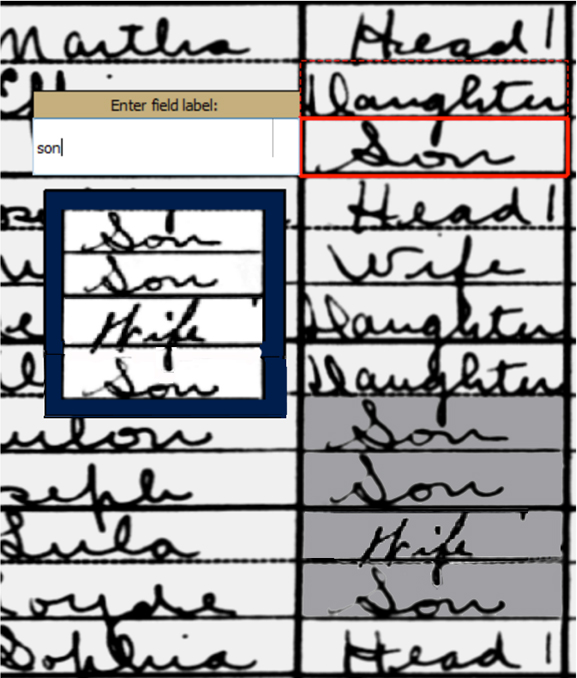
\includegraphics[width=\textwidth]{ii_ex_new_a}
    		\caption{A small window shows matching words from the column. The user can get rid of bad matches (e.g. ``Wife'') by clicking on them.}
    	\end{subfigure}
    	~
    	\begin{subfigure}[t]{0.23\textwidth}
    		\centering
    		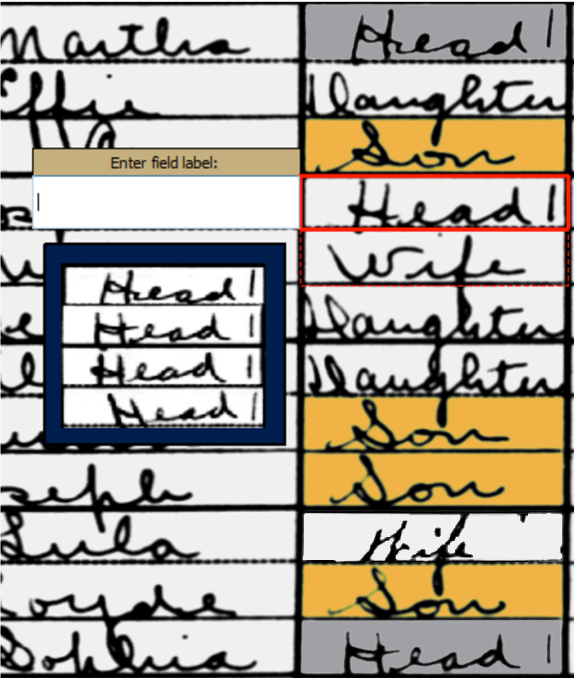
\includegraphics[width=\textwidth]{ii_ex_new_b}
    		\caption{The matched words are given the same label, indicated by the highlighting.
    		 and the red box is advanced to the next word to be transcribed.}
    	\end{subfigure}
    	\caption{Clawson's CAT system, Intelligent Indexing.
    	% a CAT system for tabular documents.
    	}
    	\label{fig:ii}
\end{figure}

\section{Using Character N-Grams}
While many words do not repeat with a high frequency in most documents, character n-grams do. We refer to a character n-gram as groups of n letters within a word. In particular, we focus on bigrams and trigrams. Let us examine the George Washington (GW) dataset \cite{GW} as an example. The most common bigram in the English language (``th'') occurs 622 times, and the 50\textsuperscript{th} most common bigram (``ur'') occurs 131 times in this dataset. This is compared to the most common word in the English language (``the'') occurring 82 times, and the 50\textsuperscript{th} most common word (``us'') occurring 9 times. Additionally, there are many words (such as ``river'') that occur only once in the dataset, but are composed of common character n-grams. 

%How can character n-grams help us transcribe? Given enough n-grams spotted in the same word, the possible transcriptions of that word are quickly reduced by constructing a simple regular expression with which to query the lexicon. To verify that this is feasible, we apply this idea to the GW dataset.

The system we propose will begin by spotting a particular n-gram (the bigram ``er'' in Fig.~\ref{fig:spotting_ex}). 
User oversight of less confident spottings will remove most of the false-positives. 
The n-grams spotted in a particular word are compiled into a regular expression that is used to query the lexicon, as seen in Fig.~\ref{fig:list}. 
If the returned list of possible trascriptions is short enough, a user can then select the correct transcription for the word with very little effort. 
Our simulation of the system follows.

If the 100 most frequent bigrams in the English language are spotted in the GW dataset with 50\% recall, 54\% of the words in the corpus can be narrowed down to 10 or fewer possible transcriptions, assuming (a) that we can correctly guess the correct number of characters we haven't spotted in the words, (b) that user oversight removing false-positives gives us 100\% precision, and (c) that we are using a 115,000 word lexicon. 
%From this list of 10 or fewer words a user can easily select the correct transcription. 
%This would be done by spotting a bigram (Fig.~\ref{fig:spotting_ex}) and passing its less confident results to users in batches, to discard the incorrect spottings.
%The different 
%Fig.~\ref{fig:spotting_ex} shows some examples the bigram ``er'' being spotted in a few words.
%We assume this is a CAT paradigm and user oversight would be able to discard any false-positives.
%Fig.~\ref{fig:list} shows how n-grams spotted in a word are being used to generate the list of possible transcriptions that would be passed to a user.
Additionally, the system will be iterative; it can learn from correct spottings and transcriptions, creating new spotting queries. Character n-grams that were missed initially will then be spotted with subsequent queries. 
If we simulate these subsequent queries achieving 50\% recall on the remaining bigrams, then by spotting the 100 bigrams again, 74\% of the corpus will be narrowed down to 10 or fewer possible transcriptions.
Some of our assumptions in our simulation are optimistic. In practice, an uncertain number of characters not spotted would result in longer lists of possible transcriptions, and some false-positives would have to be detected at the users' word-selection step, slowing down the system. We are are confident, however, that it still would be effective.


\begin{figure}
    \centering
    \begin{subfigure}[t]{0.23\textwidth}
    		\centering
    		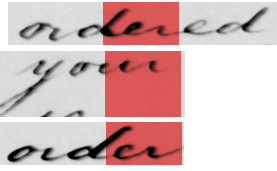
\includegraphics[height=2.7cm]{er}
    		\caption{}%Example spotting results for the bigram ``ER.'' The first word containing one true positive, the second a false positive and true positive, and the third a false positive and a false negative.}
    		\label{fig:spotting_ex}
    	\end{subfigure}
    	~
    	\begin{subfigure}[t]{0.23\textwidth}
    		\centering
    		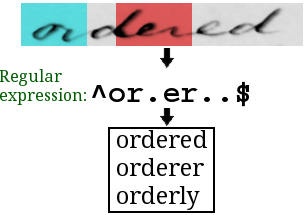
\includegraphics[height=2.7cm]{regex}
    		\caption{}%From knowing the location of the bigrams ``DE'' and ``RE,'' a regular expression can be constructed which narrows down the possible transcriptions to two words in a 32,000 word lexicon.}
    		\label{fig:list}
    	\end{subfigure}
    	\caption{(a) shows results of spotting the bigram ``er'' with our adaptation of \cite{Almazan2014}. The false positive (``ur'' in ``your'') could be removed with user oversight. (b) shows that from the bigrams ``or'' and ``er,'' a regular expression can be constructed that returns only three possible transcriptions from a 115,000 word lexicon.}
    	\label{fig:spotting}
\end{figure}

\section{Character N-Gram Spotting Experiment}
Spotting subword character n-grams is a largely unexplored area. We have run some initial tests using some word spotting techniques in the application of subword spotting to demonstrate that this is feasible. We evaluated two spotting methods: a part-structured inkball method by Howe \cite{Howe2013} and an attribute embedding method presented by Almaz\'{a}n et al.~\cite{Almazan2014}. Because these are whole word spotting methods, they are not suited to perform subword spotting without some modification. We therefore modified the code provided by Almaz\'{a}n\footnote{\url{http://github.com/almazan/watts}} and Howe\footnote{\url{http://cs.smith.edu/~nhowe/research/code/index.html#psm}}.
%\footnote{Found at \url{http://github.com/almazan/watts} and \url{http://cs.smith.edu/~nhowe/research/code/index.html#psm} respectively.}.

We used two datasets to evaluate the subword spotting performance of these methods: the George Washington dataset \cite{GW} and the IAM off-line dataset \cite{IAM}. The testing queries consisted of 10 images of each of the 20 most frequent bigrams in the English language and 5 images of each of the 10 most frequent trigrams. Query images were manually cropped from word images of the datasets. 
%\cite{Jones2004}
%\cite{Solso1979}
%There is a mismatch between methods as the attribute embedding method requires training, whereas the inkball method does not. To allow for easy comparison 
Both methods were tested using the same first fold of the testing partitions used by as Almaz\'{a}n et al.~(available with the provided code).
%All three modes of Almaz\'{a}n et al.'s method (query by string, by word, and a hybrid of both) are reported.
%Though the GW dataset is often evaluated with cross-validation due to sparsity, we did not feel this was necessary for our tests as character n-grams occur with much more frequency than words do; we used the first fold of the partitioning used by Almaz\'{a}n et al. 
The GW testing set contains 1215 word images, and the IAM testing set contains 13752 word images. Stop words were not ignored in any way. The attribute embedding method was not trained on character n-gram images but on word images.
%GW 1266 search bigrams, 295 search trigrams
%IAM 11276 search bigrams, 2722 search trigrams

%A follow-up evaluation was done using the method by Almaz\'{a}n et al.~to spot by string the 100 most frequent bigrams using both the GW and IAM datsets.

\section{Results and Conclusion}

%\begin{table}
%%\centering
%\caption{Mean-average-precision on bigrams and trigrams}
%\begin{center}
%\label{table:bigrams}
%\begin{tabular}{@{}lcccc@{}}
%\toprule
%              &\multicolumn{2}{c}{Bigrams} & \multicolumn{2}{c}{Trigrams}\\ 
%Method                         & GW      & IAM       & GW      & IAM     \\ \midrule
%Howe (by image)                & 22.11\% & 9.36\%    & 28.13\% & 6.25\%  \\ 
%Almaz\'{a}n et al.~hybrid       & 49.16\% & 24.47\%   & 67.31\% & 52.79\% \\ 
%Almaz\'{a}n et al.~by string    & 49.16\% & 24.47\%   & 63.33\% & 52.55\% \\ 
%Almaz\'{a}n et al.~by image     & 32.10\% & 19.65\%   & 65.60\% & 44.64\%    
%\end{tabular}
%\end{center}
%\end{table}

\begin{table}
%\centering 
\caption{Mean-average-precision on 20 most frequent bigrams and 10 most frequent trigrams}
\begin{center}
\label{table:bigrams}
\begin{tabular}{@{}lcccc@{}}
\toprule
              &\multicolumn{2}{c}{Bigrams} & \multicolumn{2}{c}{Trigrams}\\ 
Method                         & GW      & IAM       & GW      & IAM     \\ \midrule
%Howe one-direction scoring     & 17.45\% & 9.15\%    & 22.87\% & 5.79\%  \\ 
Howe (query by image)                & 22.11\% & 9.36\%    & 28.13\% & 6.25\%  \\ 
Almaz\'{a}n et al.~query by image     & 40.67\% & 23.10\%   & 69.79\% & 42.91\% \\
Almaz\'{a}n et al.~query by string    & 64.20\% & 32.99\%   & 65.05\% & 48.87\% \\ 
Almaz\'{a}n et al.~hybrid query       & 64.32\% & 33.04\%   & 72.38\% & 49.81\%  
\end{tabular}
\end{center}
\end{table}
%unigram query by stirng 45.31% mAP

%\begin{table}
%%\centering 
%\caption{Subword spotting results using Almaz\'{a}n et al.~to query by string on the 100 most frequent bigrams.}
%\begin{center}
%\label{table:res100}
%\begin{tabular}{@{}lcc@{}}

%Dataset: & GW      & IAM\\ \midrule
%mAP:     & 45.27\% & 20.65\%
%\end{tabular}
%\end{center}
%\end{table}


Table \ref{table:bigrams} shows the results of the experiment. The method by Almaz\'{a}n et al.~achieved a mean-average-precision that is acceptable for a CAT system as a user can discard incorrect spotting results.
%The difference between the results of spotting the top 20 versus top 100 bigrams is likely because there were fewer instances of the less common bigrams in the training set. For the GW dataset there are on average 98 training instances for each of the top 20 most frequent bigrams and only 33 training instances for the next 80 bigrams; in query by string, the spotting is wholly dependent on these.
%It may also indicates certain n-grams might be easier to spot than others due to the shape of the bigram.
The 50\% recall rate used in the simulation was drawn from these results (Almaz\'{a}n et al.~hybrid query of bigrams on GW dataset); it will roughly correspond to 66\% precision. This is an acceptable rate as users will be discarding less than half of the bigram spotting results; however, it would be desirable to relieve more of the user burden by having an improved spotting method.
%The success of the the query by string mode of the method by Almaz\'{a}n et al.~may be attributed to there being many training instances of
We are confident better subword spotting accuracy than we report will be able to be achieved with further work as we have used only na\"{i}ve adaptations of whole-word spotting approaches.

Clawson and Zagoris et al.~have shown that word spotting can create CAT systems that leverage word repetition to outperform manual transcription. We argue, and our preliminary results indicate, that character n-gram spotting can be used to construct a CAT system able to perform well independent of word repetition. A user's oversight will allow precise n-gram spotting results. As more n-grams are spotted in a particular word, its list of possible transcriptions is constrained so that a user can easily select the correct one. As spotting results are harvested to create more queries, more n-grams will be spotted, and more of the document will be transcribed.





% trigger a \newpage just before the given reference
% number - used to balance the columns on the last page
% adjust value as needed - may need to be readjusted if
% the document is modified later
%\IEEEtriggeratref{8}
% The "triggered" command can be changed if desired:
%\IEEEtriggercmd{\enlargethispage{-5in}}

% references section

% can use a bibliography generated by BibTeX as a .bbl file
% BibTeX documentation can be easily obtained at:
% http://mirror.ctan.org/biblio/bibtex/contrib/doc/
% The IEEEtran BibTeX style support page is at:
% http://www.michaelshell.org/tex/ieeetran/bibtex/
\bibliographystyle{IEEEtran}
% argument is your BibTeX string definitions and bibliography database(s)
\bibliography{IEEEabrv,bib}
%
%\bibliography{bib}
% <OR> manually copy in the resultant .bbl file
% set second argument of \begin to the number of references
% (used to reserve space for the reference number labels box)
%\begin{thebibliography}{1}

%\bibitem{IEEEhowto:kopka}
%H.~Kopka and P.~W. Daly, \emph{A Guide to \LaTeX}, 3rd~ed.\hskip 1em plus
%  0.5em minus 0.4em\relax Harlow, England: Addison-Wesley, 1999.

%\end{thebibliography}




% that's all folks
\end{document}


